\documentclass[xcolor=svgnames,english,presentation]{beamer}
%\documentclass[xcolor=svgnames,english,handout]{beamer}

%\usepackage{againframetitle}
%\aftOptions{style=NumberedLast}

\usepackage{graphics}
\usepackage{graphicx}
\usepackage{tabularx}

\usepackage{tikz}
\usepackage{pgfplots}

\graphicspath{{.}{pics/}}

% AALTO COLORS
\definecolor{aaltoyellow}{RGB}{254,203,00}  % FECB00
\definecolor{aaltored}{RGB}{237,41,57}      % ED2939
\definecolor{aaltoblue}{RGB}{00,101,189}    % 0065BD
\definecolor{aaltogray}{RGB}{146,139,129}   % 928B81
\definecolor{aaltolgreen}{RGB}{105,190,40}  % 69BE28
\definecolor{aaltodgreen}{RGB}{00,155,58}   % 009B3A
\definecolor{aaltocyan}{RGB}{00,168,180}    % 00A8B4
\definecolor{aaltopurple}{RGB}{102,57,183}  % 6639B7
\definecolor{aaltomagenta}{RGB}{177,05,157} % B1059D
\definecolor{aaltoorange}{RGB}{255,121,00}  % FF7900
\definecolor{aaltogreen}{RGB}{00,155,58}   % 009B3A

\useoutertheme{infolines} 
\setbeamertemplate{navigation symbols}{} 
%\usetheme{Marburg}
%\usetheme{Copenhagen}
%\usetheme{Frankfurt}
%\usetheme{Warsaw}
%\usetheme{Dresden}
\usetheme{Madrid}
%\setbeamercolor{structure}{fg=CadetBlue!90!black} 
\setbeamercolor{structure}{fg=aaltogreen!100!black} 
%\usecolortheme[overlystylish]{albatross}

\mode<presentation>
{
  \setbeamercovered{transparent}
}

\mode<handout>
{
  \beamertemplatesolidbackgroundcolor{black!5}
}

\usepackage[english]{babel}
%\usepackage[finnish]{babel}
% or whatever

\usepackage[latin1]{inputenc}
% or whatever

% \usepackage{times}
% \usepackage[T1]{fontenc}
% Or whatever. Note that the encoding and the font should match. If T1
% does not look nice, try deleting the line with the fontenc.

%\usepackage{amsmath,amsfonts}
%\usepackage[subscriptcorrection]{mtpro2}

\usepackage{upgreek}
\usepackage{amsmath,amsfonts,amssymb,amsthm}
% \usepackage{amsmath,amsfonts,amssymb,amsthm,mathrsfs}
% \usepackage{mathptmx}


%\title[Multiple Target Population Estimation]{A
%  Multiple Target Tracking Approach for Statistical Estimation of
%  Large Predator Population}

\newcommand{\balert}[1]{\textcolor{blue}{#1}}


\title{The Julia Language}
\subtitle{With a performance comparison in Kalman filtering}


%\subtitle
%{Presentation Subtitle} % (optional)

\author{Simo S\"arkk\"a}
% - Use the \inst{?} command only if the authors have different
%   affiliation.

\institute{Aalto University} % (optional, but mostly needed)

% - Use the \inst command only if there are several affiliations.
% - Keep it simple, no one is interested in your street address.

\date{November 10, 2015}

%\subject{Talks}
% This is only inserted into the PDF information catalog. Can be left
% out. 


% If you have a file called "university-logo-filename.xxx", where xxx
% is a graphic format that can be processed by latex or pdflatex,
% resp., then you can add a logo as follows:

%\pgfdeclareimage[height=0.5cm]{university-logo-small}{aalto_logo}
%\pgfdeclareimage[height=2cm]{university-logo-big}{aalto_logo}

% Delete this, if you do not want the table of contents to pop up at
% the beginning of each subsection:
\AtBeginSection[]
{
  \begin{frame}<beamer>
    \frametitle{Contents}
    \tableofcontents[currentsection]
  \end{frame}
}


% If you wish to uncover everything in a step-wise fashion, uncomment
% the following command: 

%\beamerdefaultoverlayspecification{<+->}

\begin{document}

%\logo{\pgfuseimage{university-logo-big}}

\begin{frame}
  \titlepage
\end{frame}

%\logo{\pgfuseimage{university-logo-small}}

%\begin{frame}
%  \frametitle{Contents}
%  \tableofcontents[pausesections]
%\end{frame}

\begin{frame}
  \frametitle{What is Julia?}

  \begin{itemize}[<+->]       
  \item Open-source \alert{programming language} for technical computing.
  \item Very \alert{Matlab-like} syntax.
  \item Interpreted language with a builtin \alert{JIT-compiler}.
  \item \alert{Fast program execution} -- closer to C than Matlab (they say).
  \item \alert{Modern programming concepts} found in Python and Lisp, but not in Matlab.
  \item \alert{Multiple dispatching} (kind of polymorphism).
  \item \alert{Operator overloading} (operators and functions).
  \begin{itemize}[<+->]       
  \item[$\Rightarrow$] {\it Demo}
  \end{itemize}
  \end{itemize}

\end{frame}

\begin{frame}
  \frametitle{Performance I}
  \centering
  Performance comparison from \url{http://julialang.org/}: 

  \vspace{0.5cm}

  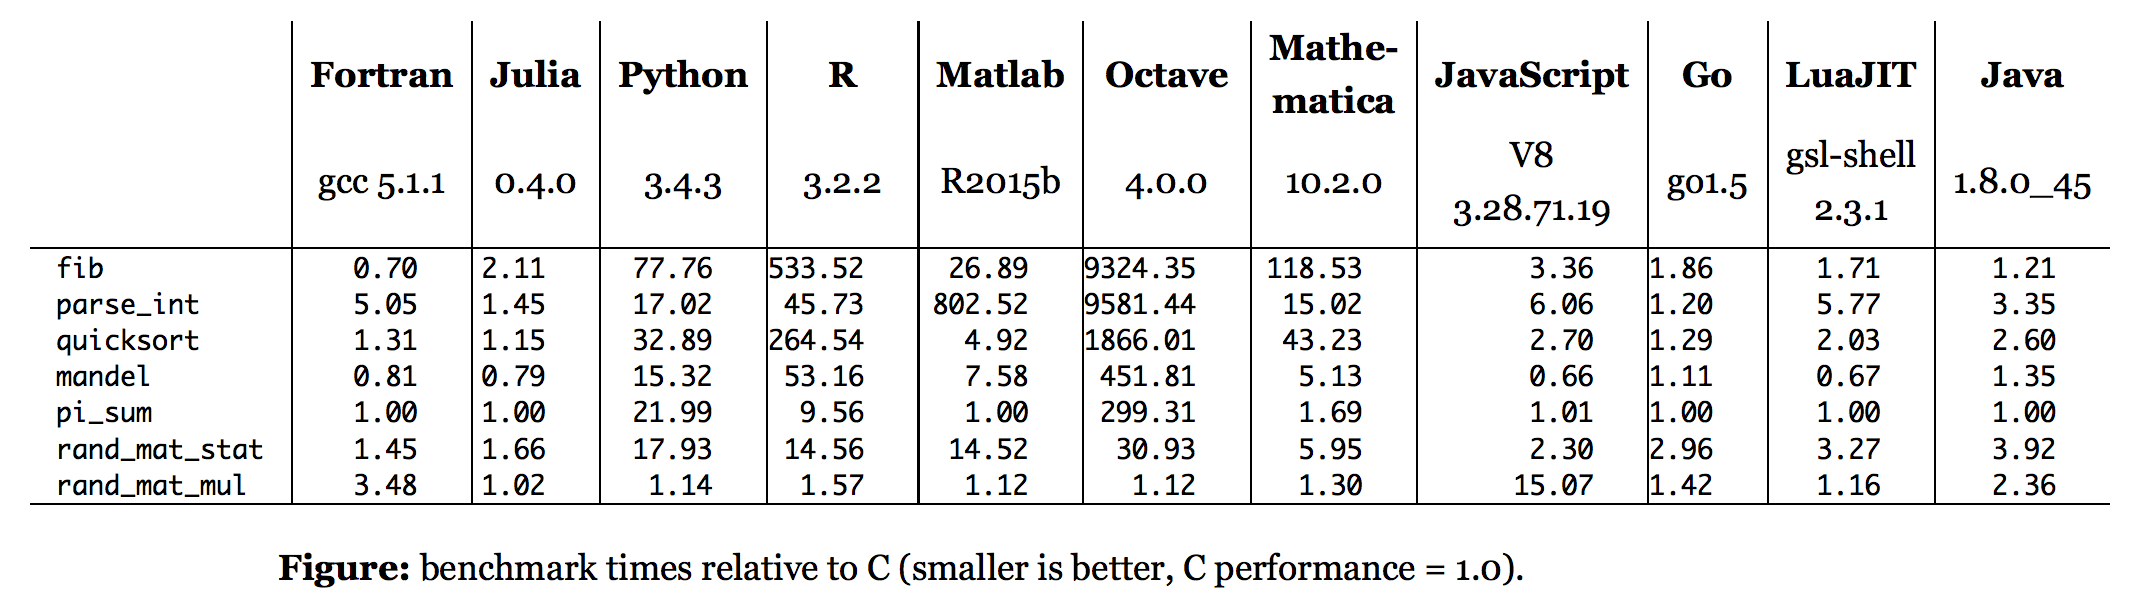
\includegraphics[width=\textwidth]{perf}
\end{frame}

\begin{frame}
  \frametitle{Performance II}
  \centering
  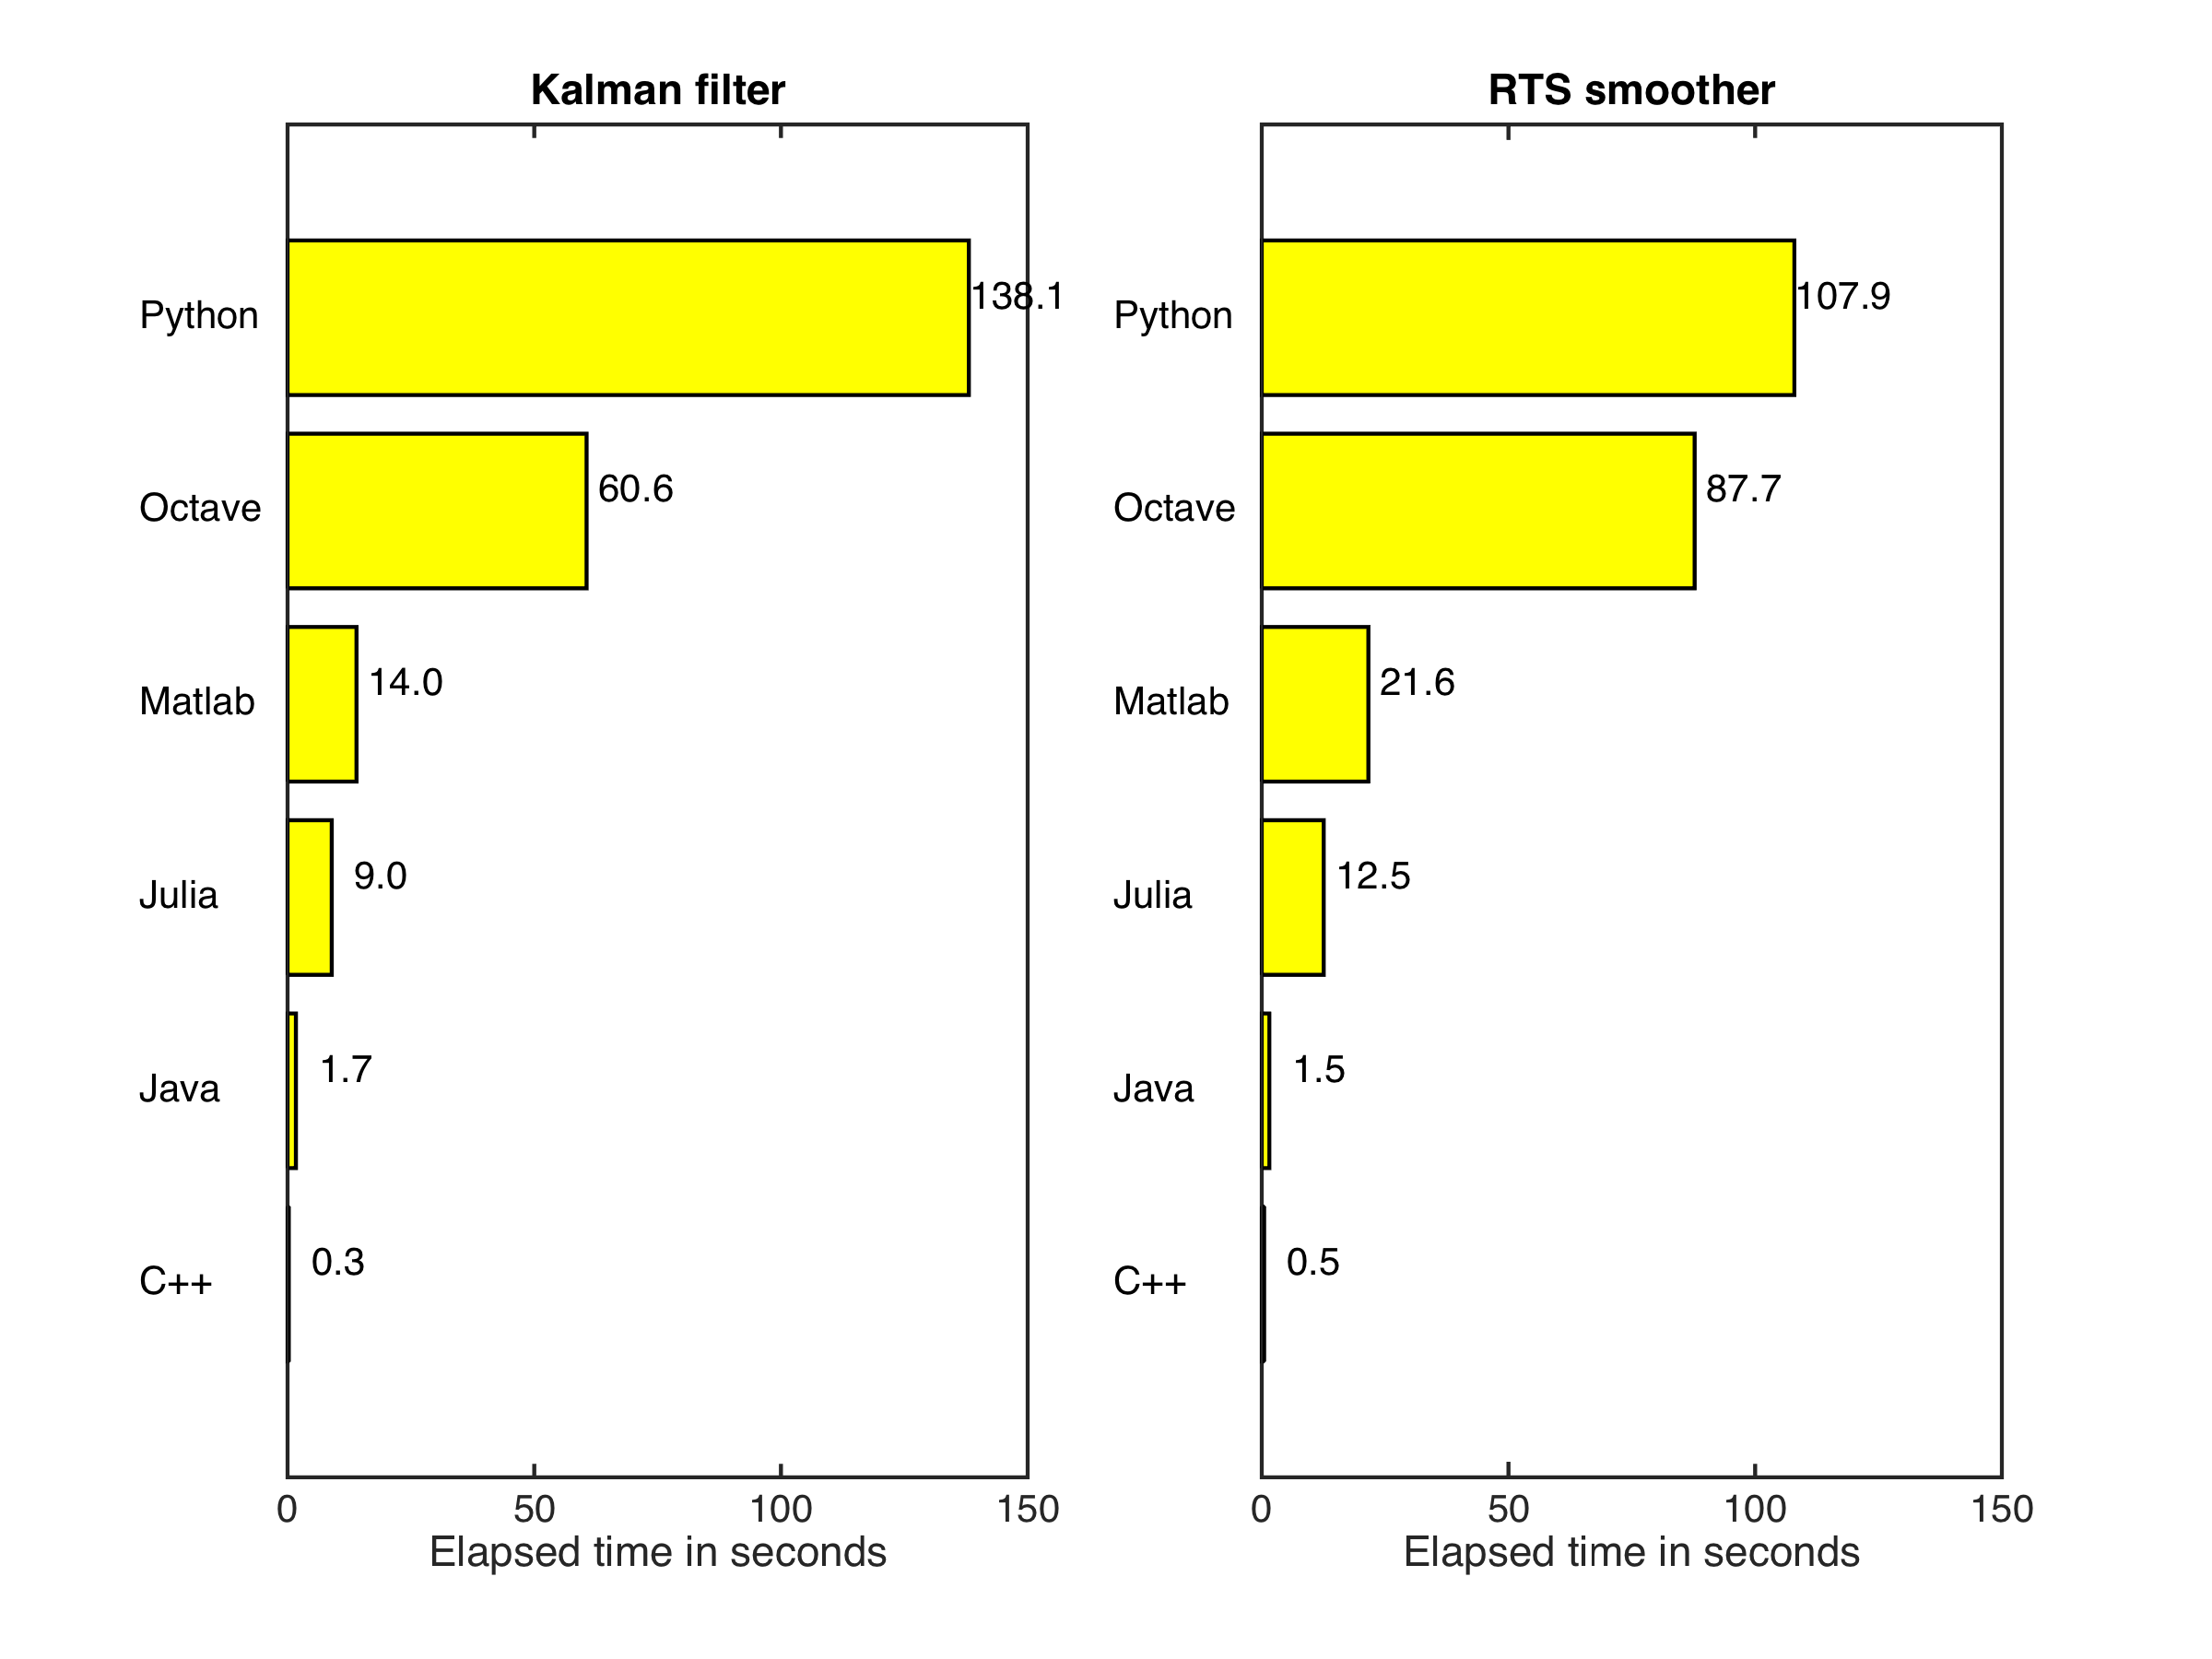
\includegraphics[width=0.7\textwidth]{kf-benchmark/times}

  \alert{Relative computation time (filter + smoother):}

  \begin{tabular}{|c|c|c|c|c|c|}
  \hline
  {\bf C++}     & {\bf Java}    & {\bf Julia}   & {\bf Matlab}  & {\bf Octave}  & {\bf Python}  \\ 
  \hline
1       & 4       & 12      & 48      & 199     & 304 \\
\hline
  \end{tabular}
\end{frame}

\begin{frame}
  \frametitle{Quick practical experiences}

  \begin{itemize}[<+->]
  \item[\textcolor{green}\checkmark] \alert{Transliteration from Matlab} is very easy (with performance catches).
  \item[\textcolor{green}\checkmark] Faster than \alert{Matlab}, but loses to \alert{C++ and Java}.
  \item[\textcolor{green}\checkmark] Much faster than \alert{Python or Octave} (no surprise).
  \item[\textcolor{green}\checkmark] Some \alert{good programming features} (proper lists, functional programming, multiple dispaching, \ldots).
  \item[\textcolor{red}\checkmark] \alert{No objects or classes!}
  \item[\textcolor{red}\checkmark] Programming environment quite \alert{clumsy to get working}.
  \item[\textcolor{red}\checkmark] \alert{Plotting features} are just awful.
  \item[\textcolor{red}\checkmark] No proper \alert{IDEs}.
  \begin{itemize}[<+->]       
  \item[$\Rightarrow$] {\it Should I switch to it?} -- \alert{Not for now.}
  \end{itemize}
  \end{itemize}

\end{frame}

\end{document}

